\documentclass[12pt]{article}

\usepackage{listings}
\usepackage{fancyhdr}
\pagestyle{fancy}
\usepackage{indentfirst}
\usepackage{layout}
\usepackage{hanging}
\usepackage{setspace}
\usepackage{mathtools}
\usepackage{graphicx}

\def\tit{Azul AI: Report}
\def\term{Fall 2019}
\def\auths{Nick Faro \& Turab Jafri \& Joshua Larkin}
\def\course{B351}

\doublespacing

\lhead{\term}
\chead{\tit}
\rhead{\thepage}
\cfoot{}

\title{
    \vspace{2in}
    \textmd{\textbf{\tit}}\\
    \normalsize\vspace{0.1in}\small{\course \ : \term }\\
    \vspace{0.1in}\large{\textit{\auths}}
    \vspace{3in}
}

\date{}

\renewcommand\headrulewidth{0.4pt}
\fancyheadoffset{0.5 cm}

\oddsidemargin 0pt
\evensidemargin 0pt
\topmargin -.3in
\headsep 20pt
%\footskip 20pt
\textheight 8.5in
\textwidth 6.25in

\setlength\topmargin{0pt}
\addtolength\topmargin{-\headheight}
\addtolength\topmargin{-\headsep}
\setlength\oddsidemargin{0pt}
\setlength\textwidth{\paperwidth}
\addtolength\textwidth{-2in}
\setlength\textheight{\paperheight}
\addtolength\textheight{-2in}

\begin{document}

\maketitle
\pagebreak

\section{Problem Space}

\begin{figure}
    \begin{center}
        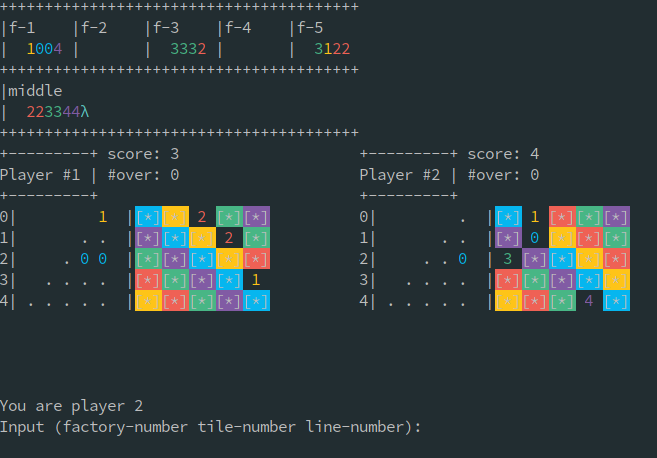
\includegraphics[width=79mm]{images/i3.png}
        \caption{Example boards; for each player, staging lines are on the left and wall is on the right}
        \label{i3}
    \end{center}
\end{figure}

Azul is a board game that comes with player boards, factories and tiles. 
The player boards have three sections: scoring, staging and the wall. 
The wall is a $5 \times 5$ Latin square, characterized by $5$ colors. 
There are $100$ tiles, $20$ of each color: black, blue, red, orange, light-blue. 
There are 9 factories total, but 2-player games only use 5 of them; 3-player games use 7 and 4-player games use all 9. 


A each row of the wall has a certain number of tiles that must be acquired to fill it, and these tiles
are color coordinated.  Players gather tiles by placing one color of tile in a staging row, then when the row is filled and the round is over, the player can place one of those tiles onto their wall -- this scores them a point.

The game is over when a row of the wall has been filled with 5 tiles. 


In Figure 1,  Player 1 needs one more blue tile to be placed in their middle staging line.
They cannot place a tile of a different color in this line, meaning that once a staging 
line has some color of tile in it, the rest of the tiles in that line need to be the 
same color. Since Player 2 can take the 2 blue tiles from the first factory 
-- filling their third staging line -- Player 1 cannot take any blue tiles. 
This means the blue tiles they have started will remain there into the next 
round (they cannot be scored this round).

When a player pick up tiles from a factory, they pick up all the tiles of one color (your choice) and place those in their staging area (a free line of their choice). 
That is one turn. Players take turns until there are no more tiles left in the factories.

Once tiles are taken from a factory, the remaining tiles (those of different color than the chosen tile) are swept
into the middle factory, which accumulates the leftover tiles.
If a player takes more tiles than they can place in a single staging row, they must place the remaining
tiles in your overflow row. The overflow row has the following scores:
$$-1, -1, -2, -2, -2, -3, -3$$
In our implementation, we just keep a count $c$ of the overflow tiles and compute the overflow score by taking the
sum of the first $c$ tiles from the row shown above.
To see how an overflow could occur, suppose Player 1 tried to place 2 blue tiles on staging line 2 in Figure 1.
This causes an overflow of 1 tile, therefore, the player will lose 1 point when their score is computed.
If they had 3 over-flown tiles, they would lose 4 points. 

\begin{figure}
    \begin{center}
        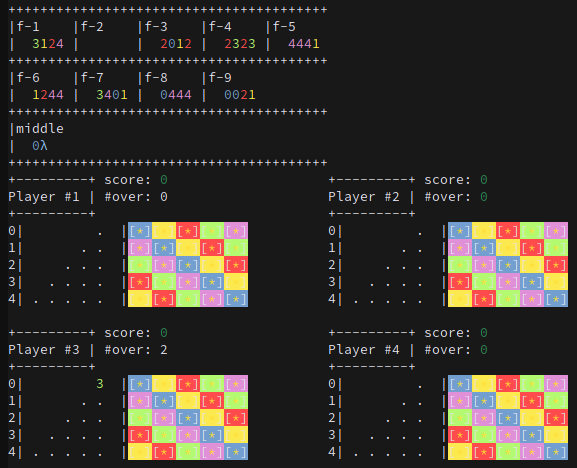
\includegraphics[width=90mm]{images/i2.png}
        \caption{Example of Azul's beginning state. Player 3 went first, took the 3 green tiles from factory 2 and placed them
                 on staging row 0. Since only 1 tile can go there, the remaining 2 green tiles go to the overflow, and
                 the remaining tiles in factory 2 are moved to the middle factory (in this case, it was just a single blue tile).}
        \label{i2}
    \end{center}
\end{figure}


Scoring begins when factories run out of tiles. If a player filled a staging row, 
they place the tile in the same row as the staging line on the spot of the wall that matches the color of the tile. 
Players get one point for placing a tile by itself, but if the tile is vertically or horizontally adjacent to
other tiles, the player sums the length of the chains it makes (in all four directions) and that is the score for the tile.
Score is marked on each player's board, and everyone's score is known to everyone else.
The last round of a game is when a player stages a tile that will be the fifth tile
in a row on their board. Once there are no more tiles left in that round, the game is over.

The challenges of Azul are very nuanced. If a player wants two blue tiles, they may have multiple factories they could take from,
but which one they do will affect the game for the rest of the players. So if another player were collecting red tiles, and needed 3 more,
they would not take blue tiles from a factory with some red tiles on it, because that
would help the other player get more red tiles -- because they would be moved to the middle factory. 

Another example is the fifth row.
Collecting 5 tiles of the same color can take time and a lot of strategy because there are not always 5 tiles of a
certain color in the distribution for the round.

Lastly, the game has bonuses: if a player places 5 tiles on their wall in a vertical column they get 7 bonus points, if they get $5$ in a row they get 2 points and if they collect 5 of a certain color you get 10 bonus points. 

There is one other variation of Azul that we have not worked with, which has a board
with no specified colors on the wall. That is, players decide where a tile goes on their wall precisely.
In the standard game the wall is pre-programmed to expect certain colors
in certain spots on the wall. In this variant the wall must have the same property that a color does appears only once in its row and column.

\section{Modeling Human Thought Processes}

%Modeling Human Thought Process:
%
%This section can appear before your Methods section.
%This section is rather vague. A good goal is to outline how humans think about Azul, using more formal language than you currently do, and explain what you think the key features of the human thought process are.
%

When people play Azul, they have to consider how they will fill in their wall.
Placing tiles in chains on the wall is the best way to score highly.
One strategy with this in mind is to start from the upper-left or upper-right corner and build out towards the center of the wall.
Another strategy is to try and build a three-by-three square in the center of the
wall and build towards the edges from there.

The fifth staging line is the most challenging to fill, because it requires
five tiles of the same color. More often than not, the color distribution is so that
there is not more than five of a given color spread across the factories.
So if a competitor were to take some of the same color a player wants for their fifth stage line, they will not be able to fill their desired staging line.
One strategy here is to gather tiles on the fifth stage line without trying to complete it by the current round's end, and instead finish other
staging lines. Then in the next round, finishing the fifth line will be easier.
If there is a color that the other players seem to not want, a player can also try to
fill in the fifth line using that color, just to get tiles placed on the fifth row 
of their board's wall.

Towards the end of the round, it is important for a player to know which 
tiles they can take, how many they can take, and to figure out who will have the last move. This allows the player to reverse engineering turns and decide if they are 
in any kind of danger. This means avoiding having to take several tiles of the same color
from the middle -- which is usually the last factory to be depleted of tiles. 

Consider this two-player scenario: Player 1 (P1) has 2 red tiles in their third staging line and an empty first staging line.
There are 2 red tiles on factory 1, and 3 red tiles in the middle factory.
These are the only factories left. Also on factory 1 are a blue tile and a black tile, and
the middle factory also has two black tiles.
It is P1's turn and they have choices.
If they take the 2 red tiles from factory 1, they take 1 red into overflow.
If they take the 3 red tiles from the middle, they take 2 red into overflow.
If they take the blue tile from factory 1, Player 2 chooses the black tiles
from the middle, then P1 must take 5 red tiles, 4 of them going to overflow.

The best choice is the first, because Player 1 reduces the overflow they must take, and
leave them-self options to take either the blue or the black on their next turn.
This highlights the ability to predict your opponents moves.




\section{Techniques}

%Techniques:
%
%Your techniques are a good start but we need more details here. Thank you for including the time and memory complexity.
%Your methods do not make any mention of the game's long-term strategy. I hope you will be at least touching on this in your final version.
%

We have implemented a generalized version of minimax -- meaning it works on more than two players.
We have a heuristic function that predicts scores for each tile in the staging area and calculates potential bonus for such placements.
The game's long-term strategy would include being more aggressive by making people take error, trying to get bonuses and being more strategic 
with when to take tiles in certain stage lines. One thing to avoid over the long-term is ending rounds with 
incomplete staging lines, because it limits the tiles a player can take in the subsequent round(s). Remark: this is good for 
filling in the fifth staging line but is not a good strategy in general.

The extended minimax does not return a best move and a best value, but instead returns a best move and a list of best 
values -- each index of the list refers to a player and the value at that index is their best value.
On updating this list, we consider the current player (whoever's turn it is) against
the remaining players. We have a few different methods of computing the best value for
the current player. They all involve taking the difference of the current player's score and a computation of the remaining players' scores. 
This computation has different instances, once as a sum, once as an average, and one as the max of the competitors' scores.

We have also made our program faster by filtering possible moves before considering them in the extended minimax algorithm. We have varied the number of moves to consider, and 15
is the best we have worked with so far. This technique was inspired by the AI implemented in the online implementation of Azul called Rojo, which greedily plays the move the seems to score the most points. We pick a few of such moves and perform the minimax algorithm on it.

The time complexity of minimax is $O(b^m)$ and the space complexity is $O(b\times m)$, where $b$ is the number of
legal moves at each point and $m$ is the maximum depth of the tree.

The limitation of this algorithm is the large search space of moves
(an upper bound of 144 different potential moves per turn).
This follows from $4$ possible colors at $6$ possible factories giving $24$ choices of tile, and $6$ possible staging lines to place on gives $144$ possible moves.
Our current implementation performs minimax at a depth of 3,
but with move filtering, we can go to higher depths with the risk of filtering out the most optimal move.
Other implementations of Azul AIs use a Monte-Carlo tree search, but we did not pursue this method.

\section{Empirical Analysis}

% Empirical Analysis:
%
% What will you be comparing? Will you use Rojo as a baseline? Random player?
% Either versus other algorithms or in different scenarios (ideally both)

Currently we do not have results we are ready to discuss.

\section{Next}

Our current AI uses a naive approach to score game states and to rank moves. Future work would be to improve these two
aspects of our AI.

To improve our state scoring heuristic, there are multiple observations we can consider. 
First, we can try to predict which staging line can get us a high score by examining the player's wall 
and the current state of factories. Our current AI just increments the score by one for a staging line that is missing 
one more tile from being fully filled.
A better approach would be to first check how much score can we gain by filling the whole staging line,
and then predicting the possibility of filling the line based on the factory states. This way, the AI will be
intelligent enough to avoid picking majority of
the moves on staging line 0 and 1.

Another approach is to adopt different scoring strategies when we approach the last round. Our current AI is not intelligent enough
to realize that it is playing the last round,
and a better approach would be to rank board states that rely on filling up a staging line in the
future rounds lower than boards that can fill staging lines in the current round. For example, 
an intelligent player would try to fill up staging lines completely
in the last round instead of filling them partially, expecting
to fill them in the future.

To improve our move-ranking strategy, we have two options that we could try in the future. 
First, we can try to do exactly what Rojo does to greedily pick a single best move.
Instead of just one, we can pick the top $k$ best moves, and perform minimax on only those moves.
Our current approach tries something similar but does not do all the computations that Rojo does.
Another approach would be to use our heuristic function and see how well the move scores.
We tried doing this in our current implementation, but since our heuristic is naive, it actually made our AI
perform worse than before. Once a better heuristic is implemented, we expect this strategy to improve the move-filtering process.


%Next:
%
%Discussion and future directions belong immediately after the Methods section.
%It is not clear whether this section is referring to changes you will make
%by next week or future work for after this semester.

%Explain how our work could be expanded or improved

\section{Acknowledgments}

In the development of our AI, we discovered an online implementation of Azul called Rojo (http://boardwebgames.com/rojo/), written by Jan-Dirk van Dingenen. Its code was unobfuscated and available online. We ported the algorithm used by Rojo to our implementation of the game for use as a comparison metric against our own AI. We do not use any part of its implementation in our AI.

The Rojo algorithm works by greedily selecting the move which could result in the highest score, including bonus. It easily beats a function that just generates random moves, and can also beat inexperienced players.

\end{document}
